\subsection{Simple Properties}
\begin{frame}
  \frametitle{Simple Properties}
  \begin{itemize}
\vfill
  \item NP-complete (CuSP is a particular case of CECSP)
\vfill
\pause
  \item scheduling a task at $\bmax$ during $\inter$ gives the higher energy amount ($f_i$ is non decreasing)
\vfill
\end{itemize}
\begin{center}
  \begin{tikzpicture}
    [yscale=0.6]
    [inner sep=0]
    \node (O) at (0,0) {};
    \node (T) [right of=O,node distance=4cm] {};
    \node (t1) [right of =O, node distance=1cm] {};
    \node (t2) [right of =t1, node distance=2cm] {};
    \draw[pattern=north west lines] (t1) rectangle (3,2.5);
    \draw[dashed,gray!40!black!40] (0,2.5) -- (4,2.5) node[right] {$\bmax$};
    
    \draw[red,dashed] (t1) node[below] {$t_1$}-- (1,3);
    \draw[red,dashed] (t2) node[below] {$t_2$} -- (3,3);
    \draw[->] (O) -- (T);
  \end{tikzpicture}
\end{center}
\pause
\vfill
  \begin{block}{Notations}
    \begin{itemize}
    \item the latest start time of $i$ as $lst_i=let_i-\frac{W_i}{f_i(\bmax)}$
    \item and the earliest end time of $i$ as $eet_i=est_i+\frac{W_i}{f_i(\bmax)}$
    \end{itemize}
  \end{block}
\vfill
\pause

  $\Rightarrow$ a task can start in $\inter[est_i][lst_i]$ and end in $\inter[eet_i][let_i]$
\vfill
\end{frame}
\subsection{Non-integer solution}
\begin{frame}
  \frametitle{Non-integer solution}
  \vfill
  \begin{itemize}
  \item   Instances with integer data can have only non-integer solution.
  \end{itemize}
  \vfill
\pause

  \begin{center}
    \begin{tabularx}{10cm}{|>{\centering\arraybackslash}p{0.6cm}|
        *5{>{\centering\arraybackslash}X}>{\centering\arraybackslash}p{2cm}|}
      \hline
      $i$ & $r_i$ & $d_i$ & $W_i$ & $\bmin$ & $\bmax$ & $f_i(b_i(t))$ \\
      \hline
      $1$ & $0$ & $2$ & $3$ & $1$ & $2$ & $b_i(t)$\\
      $2$ & $1$ & $3$ & $3$ & $1$ & $2$ & $b_i(t)$\\
      \hline
    \end{tabularx}
  \end{center}
  \vfill
\pause

  \centering
  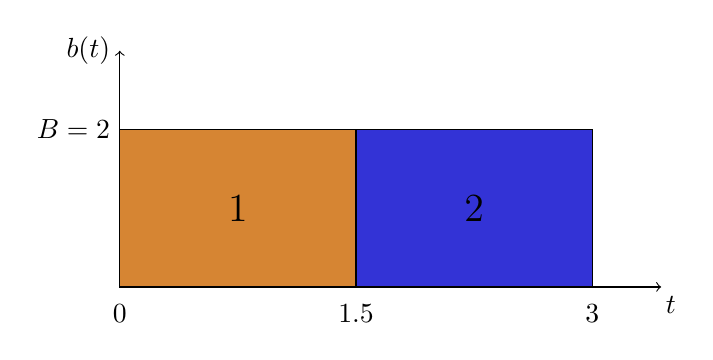
\begin{tikzpicture}
    [xscale=2]
    \node (O) at (0,0) {} node[below=0.1cm] {$0$};
    \draw (1.5,0)  node[below=0.1cm] {$1.5$};
    \draw (3,0) node[below=0.1cm] {$3$};
    \node (T) at (3.5,0) {};
    \draw(0,2)  node[left,node
    distance=1.5pt] {$B=2$}; 
    \draw[fill=orange!80!black!80] (O) rectangle (1.5,2);
    \draw[fill=blue!80!black!80] (1.5,2) rectangle (3,0);
    \draw[->] (0,0) -- (T) node[below] {$t$};
    \draw[->] (0,0) -- (0,3) node[left] {$b(t)$};
    
    \node at (0.75,1) {\Large 1};
    \node at (2.25,1) {\Large 2};
  \end{tikzpicture}
  \vfill  
\end{frame}

\subsection{Piecewise Constant Resource Allocation}
\begin{frame}{Piecewise Constant Resource Allocation}
  \begin{theorem}
    Any solution of \only<1-8>{\textcolor{blue!80!black!80}{CECSP$_{lin}$}}
    \only<9->{\textcolor{red!80!black!80}{CECSP$_{cpwl}$}} and can be transformed in a solution
    where $\forall i \in A,\ b_i(t)$ is piecewise constant.  
  \end{theorem}
  \onslide<2->{
    \begin{proof}[Proof (Sketch)]
      \begin{columns}
        \begin{column}{0.55\linewidth}
          \begin{overlayarea}{\textwidth}{4cm}
            \only<2-10>{
              \begin{itemize}
              \item<3-> $(t_q)$: series of start and end times
                \vspace{0.2cm}
              \item<4-> in $\inter[t_q][t_{q+1}]$, $b'_i(t)$ is set to the mean value of $b_i(t)$ over this interval
              \end{itemize}
              \begin{overlayarea}{\textwidth}{0.5cm}
                \only<8>{	
                  \begin{itemize}
                  \item same resource and {\color{blue!80!black!80}same} energy
                  \end{itemize}
                }
                \only<9>{ \begin{itemize}
                  \item same resource and {\color{red!80!black!80}more} energy\footnote{Jensen,
                      Sur les fonctions convexes et les in{\'e}galit{\'e}s entre les
                      valeurs moyennes, 1906.}
                  \end{itemize}}
                \only<10->{\begin{itemize}
                  \item $et_i=$ value for which required energy is received        
                  \end{itemize}}
              \end{overlayarea}}
            \only<11>{
              \vspace{1cm}
              \begin{center}

                {\bf Remark: } We only have 

                to change $b_i(t)$ for 

                $t \in
                \cup_{i\in A} \{st_i,et_i\}$
                
              \end{center}}
          \end{overlayarea}
        \end{column}
        \begin{column}{0.45\linewidth}
          \onslide<2->{
            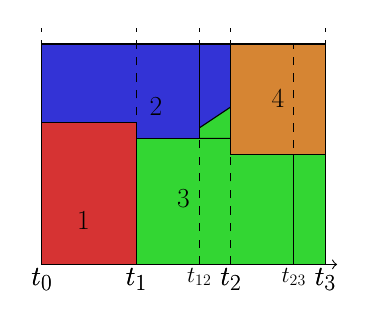
\begin{tikzpicture}
              [scale=0.4,transform shape]
              [inner sep =0]
              \node (O) at (0,0) {};
              \node (T) [right of=O,node distance=9.5cm] {};
              \onslide<2-9>{
                \fill[blue!80!black!80,draw=black] (0,3) rectangle (6,7) node[midway, right=0.8cm] { \color{black} \Huge $2$};}
              \onslide<2-4>{
                \fill[red!80!black!80,draw=black] (0,0) node[above right=1cm] { \color{black} \Huge $1$}-- (0,4) parabola bend (1.5,5) (3,4) --(3,0) -- cycle;}
              \onslide<5-9>{
                \fill[red!80!black!80,draw=black] (0,0) node[above right=1cm] {\color{black} \Huge $1$}-- (0,4.5) --(3,4.5) --(3,0) -- cycle;}
              \onslide<2-9>{
                \fill[orange!80!black!80,draw=black] (9,7) rectangle (6,2);
                \fill[orange!80!black!80] (9,7) rectangle (6,3.5) node[midway] {\color{black} \Huge $4$};}
              \onslide<2-5>{
                \fill[green!80!black!80,draw=black] (3,0) -- (9,0) -- (9,2) -- (6,5)-- (3,3)  node[below, right=2cm] { \color{black} \Huge $3$}-- cycle;}
              \onslide<6>{
                \fill[green!80!black!80,draw=black] (3,0) -- (9,0) -- (9,2) -- (6,5)-- (6,4)  node[left=1.5cm,below=1.5cm] { \color{black} \Huge $3$} --(3,4) -- cycle;
                ;}
              \onslide<7-9>{
                \fill[green!80!black!80,draw=black] (3,0) -- (9,0) -- (9,3.5) -- (6,3.5)-- (6,4)  node[left=1.5cm,below=1.5cm] { \color{black} \Huge $3$} --(3,4) -- cycle;
              }
              \draw[->] (O) -- (T);
              \onslide<10->{
                \fill[blue!80!black!80,draw=black] (0,3) rectangle (5,7) node[midway, right=0.8cm] { \color{black} \Huge $2$};
                \fill[red!80!black!80,draw=black] (0,0) node[above right=1cm] {\color{black} \Huge $1$}-- (0,4.5) --(3,4.5) --(3,0) -- cycle;
                \fill[orange!80!black!80,draw=black] (9,7) rectangle (6,3.5) node[midway] {\color{black} \Huge $4$};
                \fill[green!80!black!80,draw=black] (3,0) -- (8,0) -- (8,3.5) -- (6,3.5)-- (6,4)  node[left=1.5cm,below=1.5cm] { \color{black} \Huge $3$} --(3,4) -- cycle;
                \draw[dashed] (0,0) node[below] {\color{black} \Huge $t_0$} -- (0,7.5);
                \draw[dashed] (3,0) node[below] {\color{black} \Huge $t_1$} -- (3,7.5);
                \draw[dashed] (5,0) node[below] {\color{black}  \huge $t_{12}$} -- (5,7.5);
                \draw[dashed] (6,0) node[below] {\color{black} \Huge $t_2$} -- (6,7.5);
                \draw[dashed] (8,0) node[below] {\color{black} \huge $t_{23}$} -- (8,7);
                \draw[dashed] (9,0) node[below] {\color{black} \Huge $t_3$} -- (9,7.5);
              }       
              \onslide<3->{
                \draw[dashed] (0,0) node[below] {\color{black} \Huge $t_0$} -- (0,7.5);
                \draw[dashed] (3,0) node[below] {\color{black} \Huge $t_1$} -- (3,7.5);
                \draw[dashed] (6,0) node[below] {\color{black} \Huge $t_2$} -- (6,7.5);
                \draw[dashed] (9,0) node[below] {\color{black} \Huge $t_3$} -- (9,7.5);
              }
            \end{tikzpicture}
          }
        \end{column}
      \end{columns}
      \vspace{0.5cm}	
    \end{proof}}
\end{frame}

\subsection{Polynomial cases}
\begin{frame}{Polynomial cases}
  \vfill
  \begin{theorem}
    The CECSP, the CECSP$_{lin}$ and the CECSP$_{cpwl}$ with fixed
    task start and end times are polynomial.  
  \end{theorem}
  \vfill
\pause
 {\bf Proof (Sketch). } Only need to decide the quantity of resource
 given to tasks in each interval $[t_{q},t_{q+1}]$.


\pause
 Can be solved by a Flow-based Linear Program.
 \vfill
\pause
  \begin{theorem}
The preemptive CECSP, the preemptive CECSP$_{lin}$ and the preemptive CECSP$_{cpwl}$ are polynomial.  
  \end{theorem}
  \vfill
\pause
  
 {\bf Proof (Sketch). } Apply the Flow-based LP with $st_i=r_i$ and $et_i=d_i$.
 \vfill
\end{frame}


% \begin{frame}{counter example concave function}
%   \vfill
%     \begin{theorem}
%     Any solution of CECSP$_{cpwl}$ and can be transformed in a
%     solution where $\forall i \in A,\ b_i(t)$ is piecewise constant. 
%   \end{theorem}
%   \vfill
%   Does not apply to the case of concave efficiency function.
%   \vfill
%   {\centering
%     \begin{tikzpicture}
% \node (O) at 
%     \end{tikzpicture}
%     }
%   \vfill 
% \end{frame}

